%
% Master Thesis
% Thomas Brüggemann
%

% Common Settings
% ------------------------
\documentclass[
	a4paper,
	oneside,
	12pt,
	liststotocnumbered
]{article}
\usepackage{times}            % Times New Roman

\usepackage[utf8]{inputenc}   % utf-8
\usepackage[english]{babel}
\selectlanguage{english}
\usepackage{nicefrac}
\usepackage{latexsym}
\PassOptionsToPackage{hyphens}{url}\usepackage{hyperref}

% Title font sizes
\usepackage{titlesec}
\titleformat{\section}{\bfseries}{\thesection.}{12pt}{}
\titleformat{\subsection}{\bfseries}{\thesubsection }{12pt}{}

% Margins
\usepackage[
    top=2.5cm, 
    bottom=2.5cm, 
    left=5cm, 
    right=1cm
]{geometry} 

% Footnotes
\usepackage[hang,flushmargin]{footmisc}    
\renewcommand*{\footnotelayout}{\footnotesize} % size of text
\renewcommand{\footnotemargin}{2.2em}          % margin between text and number
\setlength{\footnotesep}{1.3em}                % space between footnotes
\setlength{\skip\footins}{2.5em}               % space between text & footnotes
\usepackage{savefnmark}

% Acronyms
\usepackage[printonlyused]{acronym}    
\renewcommand{\bflabel}[1]{{#1\hfill}}

% Page numeration oben
\usepackage{scrpage2} 
\usepackage[dvips]{color}
\clearscrheadfoot 
\chead[\pagemark]{\textcolor[gray]{0.5}{\pagemark}} 
\pagestyle{scrheadings}

% TOC, LOF, FIG Styles
\usepackage{tocloft, titletoc}  
\setlength{\cftaftertoctitleskip}{0em}
\renewcommand{\cftloftitlefont}{\bfseries}
%\renewcommand{\cftfigfont}{\bfseries}
\renewcommand{\cfttoctitlefont}{\bfseries}
\renewcommand{\cftlottitlefont}{\bfseries}
\titlecontents{section}     % set formatting for \section 
[2.3em]                     % adjust left margin
{\vspace{0.5em}}            % font formatting
{\hspace{-1.8em}.\contentslabel{0.7em}\hspace{1em}} % section label and offset
{\hspace*{-2.3em}}
{\titlerule*[1mm]{.}\contentspage}

\titlecontents{subsection}  % set formatting for \subsection 
[3em]                       % adjust left margin
{\vspace{0.5em}}            % font formatting
{\contentslabel{2.3em}}     % section label and offset
{\hspace*{-2.3em}}
{\titlerule*[1mm]{.}\contentspage}

\titlecontents{subsubsection}  % set formatting for \subsubsection 
[4.2em]                       % adjust left margin
{\vspace{0.5em}}            % font formatting
{\contentslabel{2.3em}}     % section label and offset
{\hspace*{-2.3em}}
{\titlerule*[1mm]{.}\contentspage}

\titlecontents{figure}      % set formatting for \subsection 
[2.3em]                     % adjust left margin
{\vspace{0.5em}}            % font formatting
{\contentslabel{2.3em}}     % section label and offset
{\hspace*{-2.3em}}
{\titlerule*[1mm]{.}\contentspage}

\titlecontents{table}       % set formatting for \subsection 
[3.4em]                     % adjust left margin
{\vspace{0.5em}}            % font formatting
{:\hspace*{0.9em}\contentslabel{4.5em}}     % section label and offset
{\hspace*{-2.3em}}
{\titlerule*[1mm]{.}\contentspage}


% References
\usepackage[
    bibstyle=authortitle,
    citestyle=authoryear,
    isbn=false,
    url=false,
    doi=false,
    maxcitenames=3,
    maxbibnames=30
]{biblatex}
\addbibresource{library.bib}
\let\cite\textcite

\usepackage{caption}
\usepackage{chngcntr}

% Tables
\usepackage{array}
\usepackage{xcolor}
\usepackage{longtable}
\usepackage{setspace}
\counterwithin{table}{section}
\usepackage{multirow}

% Figures
\usepackage[pdftex]{graphicx}
\graphicspath{{figures}}
\counterwithin{figure}{section}
\usepackage[absolute,overlay]{textpos}

\begin{document}

% Renews
\renewcommand{\figurename}{Fig.}
\renewcommand{\tablename}{Tab.}
\renewcommand\thefigure{\arabic{section}-\arabic{figure}}
\renewcommand\thetable{\arabic{section}-\arabic{table}}
\newcommand{\todo}[1]{\textbf{\textsc{\textcolor{red}{TODO: #1}}}}

% Variables
\newcommand{\mH}{mHealth }
\newcommand{\ap}{app provider }
\newcommand{\pp}{privacy policy }
\newcommand{\pps}{privacy policies }
\newcommand{\sca}{static code analysis }
\newcommand{\Sca}{Static code analysis }
\newcommand{\pra}{information privacy risk assessment }
\newcommand{\prfs}{information privacy risk factors }
\newcommand{\ipr}{information privacy risks }
\newcommand{\iprfs}{information privacy risk factors }
\newcommand{\iprs}{information privacy risk score }
\newcommand{\gui}{graphical user interface }
\newcommand{\ipp}{information privacy practices }
\newcommand{\Ipp}{Information privacy practices }
\newcommand{\aiprat}{automated information privacy risk assessment tool }
\newcommand{\nbc}{naive Bayes classifier }
\newcommand{\AIPRAT}{\textit{AIPRAT} }

\pagenumbering{Roman}

% ---------
% Cover pages
% ---------
\vspace*{1mm}

% Name
\thispagestyle{empty}
Thomas Brüggemann

\vspace*{23mm}

% Bacheloararbeit
\begin{center}
\textbf{
    Master Thesis
\linebreak
    im Fach Information Systems}
\end{center}

\vspace*{20mm}

% Titel
\begin{center}
\LARGE 
    Automated Information Privacy Risk Assessment of Android Health Applications
\end{center}

\vspace*{8mm}

% Themensteller
\begin{center}
    Themensteller: Prof. Dr. Ali Sunyaev
\end{center}

\vspace*{12mm}

% Vorgelegt
\begin{center}
    Vorgelegt in der Masterprüfung
\linebreak
    im Studiengang Information Systems
\linebreak
    der Wirtschafts- und Sozialwissenschaftlichen Fakultät
\linebreak
    der Universität zu Köln
\end{center}

\vspace*{30mm}

% Köln, April 2013
\begin{center}
Köln, März 2016
\end{center}




% ------------------
% Table of Contents
% ------------------
\tocloftpagestyle{scrheadings}
\tableofcontents
\newpage

% ---------------------
% Acronyms
% ---------------------
% Abkürzungsverzeichnis
\section*{Index of Abbreviations}
\addcontentsline{toc}{section}{Index of Abbreviations}
\begin{acronym}[TTTTTTTTTTTTTTTTTTTT]
	\acro{API}{Application Programming Interface}
	\acro{APK}{Android Application Package}
	\acro{DEX}{Dalvik Executable}
	\acro{DRM}{Digital Rights Management}
	\acro{GPS}{Global Positioning System}
	\acro{HTTP}{Hypertext Transfer Protocol}
	\acro{HTTPS}{Hypertext Transfer Protocol Secure}
	\acro{HTML}{Hypertext Markup Language}
	\acro{IP}{Internet Protocol}
	\acro{JAR}{Java Archive}
	\acro{JVM}{Java Virtual Machine}
    \acro{mHealth}{Mobile Health}
    \acro{NFC}{Near Field Communication}
    \acro{P3P}{Platform for Privacy Preferences}
    \acro{TCP/IP}{Transmission Control Protocol / Internet Protocol}
    \acro{URI}{Uniform Resource Identifier}
    \acro{URL}{Uniform Resource Locator}
    \acro{UUID}{Universally Unique Identifier}
    \acro{XML}{Extensible Markup Language}
\end{acronym}
\newpage

% -------------------
% List of tables
% -------------------
\listoftables
\addcontentsline{toc}{section}{List of tables}
\newpage

% -------------------
% List of figures
% -------------------
\listoffigures
\addcontentsline{toc}{section}{List of Figures}
\newpage

\normalsize
\setstretch{1,5}
\pagenumbering{arabic}

% ------
% Chapters
% ---------
\section{Introduction}

\subsection{Problem Statement}

The market for mobile phone and tablet applications (apps) has grown extensively since recent years.\footnote{See for this and the following sentence \cite{Enck2011}, p. 1.}
It is increasingly easier for companies or even single developers to create unique apps that reach millions of users around the planet via digital app stores.
This market growth affected mobile health (\acs{mHealth}) apps as well. 
More and more \mH apps are available that support the users in resolving their health-related issues and that try to remedy health-related information deficiencies. 

But receiving personal health-related information yields information privacy risks to users.
Users are asked to expose personal health-related information, e.g. information on disease symptoms or medical appointments in order to receive a tailored app that fits their needs.\footnote{See \cite{Chen2012}, p. 2.}
It remains however unclear how and where the vulnerable user information is sent, processed and stored.\footnote{See \cite{He2014}, p. 652.}

The information about these privacy related practices of app providers and their offered apps should be stated in the privacy policy document provided by the app provider.\footnote{This paragraph follows \cite{Dehling2014}, p. 11.}
Processing these \pps requires a higher level of education and time to read through large bodies of text, in order to find the relevant information. 
Additionally, the important information is hidden in legal language or is  insufficiently addressed, if at all.\footnote{See \cite{Pollach2007}, p. 104.}
Aside from data usage beyond the control of the users, it is also challenging to assess what kind of private information an app asks for, prior to the app usage. 
Users have to download the apps of interest and try them out, before it becomes clear what health-related information is processed by the app and in which  way. 
This leads to low comparability between apps. 
When users are looking for specific functionality in an \mH app, it is challenging to find the app that offers the desired functionality at an acceptable information privacy risk. 
Even if users would pursue the task of finding and comparing \mH apps of similar functionality, the high volume of apps available in the app stores\footnote{See \cite{Enck2011}, p. 1.} makes it laborious to review all of them by hand.
One way to assess \ipr of the large amount of \mH apps is to automate the review process of each individual app. 
The assessment automation can be done by downloading and analyzing the source code of each app and by tracing data leaks. 
\Sca is used in the field of informatics to analyze application source code and detect faults or vulnerabilities.\footnote{See \cite{Baca2008}, p. 79.} 
It is yet unclear how and to what degree the concepts of \sca and \pra can be combined in order to automate app assessment.
A \sca could, in theory, be used to automatically assess some of the \ipr that \mH apps pose.
Previous research has not shown how and to what degree the combination of \sca and \ipr assessment is feasible in the field of \mH app \pra and therefore the aim of this study is to explore the possibilities of static code analysis for information privacy risk assessment. 
This leads to the research question: How and to what degree can the \ipr of \mH apps be automatically assessed?
The 'degree' refers to the amount and the level of detail that \iprfs can be automatically assessed.

The automated process furthermore can help to drastically reduce the effort of reviewing each individual app and can enhance the information experience users receive while looking for mHealth apps.
Additionally, it exposes new possibilities for research in the \ipr area. 
The research could be conducted on providing solutions and best practices for further enhancing the \ipr communication of apps.

\subsection{Objectives}

The main objective of this study is to ascertain how and to what degree the assessment of \iprfs for \mH apps can be automated.
In order to reach this objective, the following sub-objectives have to be met.

The first sub-objective is to extract \iprfs from the \ipp that \cite{Dehling2016} identified and that are relevant for automated information privacy risk assessment.
As a second sub-objective we will develop strategies to identify the \iprfs within the source code of \mH apps via static code analysis.
This is necessary since it is yet unclear how and to what degree the \sca can help to identify \iprfs of \mH apps. 
Finally we will evaluate how well the automated \pra tool can identify \iprfs in comparison to two human reviewers.
In order to fully ascertain the degree \sca can identify information privacy risk factors, a manual review of the results of the \sca is necessary.

\subsection{Structure}

This work is structured in five chapters and the content can be summarized as follows. 
The previous sections of this chapter motivated the goals of this thesis by outlining the knowledge gap of how and to what degree \ipr assessment of \mH apps can be automated.

In section 2, we\footnote{Although this work is done by a single author, 'we' and 'our' respectively will be used throughout this thesis.} will give an overview over the current state of the research and lay the foundations of this thesis.
We will first highlight research regarding information privacy risk assessments and its current limitations in section 2.1.
Following in chapter 2.2, we will outline research regarding static code analysis. 
We take special interest in further possibilities \sca offers for interdisciplinary research, between technical possibilities and business informatics.
The data base for this thesis, the \ipp identified by \textcite{Dehling2016} will be introduced in chapter 2.3.

Chapter 3 focuses on the implementation and evaluation of an \aiprat.
We will explain the three phases of the implementation of the \aiprat in detail in chapter 3.1.
The following chapter 3.2 explains the process of evaluation of the \aiprat performance in comparison to two human researchers.

The next chapter, chapter 4, will present the results of the implementation and evaluation of the \aiprat.
Chapter 4.1 contains results of the three implementation phases and will also point out the challenges that occurred within the implementation phases.
The results of the evaluation of the \aiprat are presented in chapter 4.2.

The thesis closes with the 'Discussion' chapter 5. 
In chapter 5.1 we will summarize the key findings of this work and will present the contributions this work offers to current research in chapter 5.2.
The limitations this thesis is under will be presented in chapter 5.3.
The next chapter 5.4 will give an outlook towards the topics that future research could cover in relation to this work.
Finally we will conclude the thesis with a conclusion chapter 5.5.

\section{Combining Source Code Analysis with Information Privacy Risk Assessment}

\mH apps have been examined in various research studies that aim at providing insights for developers as well as for users into how private information is processed.
Privacy issues are the most impactful user complaints while using mobile apps.\footnote{See \cite{Khalid2015}, p. 5.}
Especially \mH apps deal with sensitive and vulnerable user information and therefore pose a high information privacy risk. \footnote{See \cite{Kumar2013}, p. 33.}
This encourages research to address information privacy risks.

\subsection{Information Privacy Risk Assessment}

% Definition IPR
Information privacy can be defined as the circumstance that people are able to control if, how and where information and knowledge about themselves is acquired, stored and processed.\footnote{See \cite{Fischer1998}, p. 421-422.}
In addition to mere control over the users private information, society and social structure must establish an information regulation architecture that allows people to sustainably enforce their information privacy rights.\footnote{See \cite{Solove2002}, p. 1115.}
An information privacy risk is therefore, by implication, a threat or a circumstance that disables users to enforce control over their private information.
Threats to information privacy in digital services can happen at application level (e.g. by sharing users' personal information with third-parties), as well as at communication level (e.g. by using an unencrypted data connection).\footnote{See \cite{Fischer1998}, p. 423-427.}

% mHealth context
For this thesis, we chose the context of \mH apps, since \mH are commonly handling sensitive user information and are therefore more prone to information privacy violations.\footnote{See \cite{Huckvale2015}, p.1-2.}
Research in the field of information privacy risk assessment of \mH apps has progressed, but research literature in this field is still behind its full potential.\footnote{\cite{Arora2014}, p. 143.}

Information privacy risk classification frameworks were developed to structure the problem of information privacy violation into risk types.\footnote{See for this paragraph\cite{Lewis2014}, p. 2-3.}
Risk types can range from \textit{loss of reputation}, where a \mH apps for instance display sensitive data to unauthorized viewers up to \textit{Inappropriate and irreversible clinical action}. 
The latter type would be reached by a defective algorithm within a \mH app that proposes wrong information.

Even though classifications of information privacy risks exist\footnote{See \cite{Lewis2014}, p. 1-3.} and subsequent regulations and policies have been put in place, \mH apps might not follow these regulations.\footnote{See \cite{Huckvale2015}, p. 1-2.}
A way to identify those apps, that claim to follow common regulations and policies, but secretly still collect sensitive information in inappropriate manners, is by applying special technology to the identification process.\footnote{See \cite{Huckvale2015}, p. 1-2, \cite{Arora2014}, p. 149.}

% Technical side
Research focus has been put on the technical side of information privacy violations and threats. 
It is possible to analyze the Android log files that \mH app might write data into as well as \acl{HTTP} (\acs{HTTP}) data connections to internet servers.\footnote{See \cite{Huckvale2015}, p. 2-5.}

It has been analyzed, to what degree the data storage in internal Android log files or on the memory card within a phone or tablet as well as data connections to the Internet pose threats to users information privacy.\footnote{For this and the next sentence, see \cite{He2014}, p. 645-646, 649.}
Special focus has been put on unencrypted HTTP connections that send out user information to either the app providers servers or third party services.
The assessment has been carried out using the network analysis tool \textit{Wireshark}\footnote{\url{https://web.archive.org/web/20160710141347/https://www.wireshark.org/}, visited 07/13/16.} that logs all HTTP traffic.\footnote{See \cite{He2014}, p. 649.}
Technical evaluation of mobile apps goes further, into the topics of decompilation to analyze device identification or geolocation data leaks.\footnote{See \cite{Mcclurg2012}, p. 1, 5., \cite{Enck2011}, p. 1. and \cite{Mitchell2013}, p. 6-7.}
In conclusion, decompilation is a widely used assessment technique for \ipr and data leaks.

\subsection{Static Code Analysis}

As suggested in previous research, insights from other fields of study can be used to elaborate on the assessment of information privacy risks in the \mH sector.\footnote{See \cite{Arora2014}, p. 143.}

The informatics and software development sector bears tools that could be applied to \ipr assessments of \mH apps.
One of these tools is a static code analysis.
Static code analysis refers to analysing the source code of a software without actually executing the software.\footnote{See \cite{Louridas2006}, p. 58.}

In informatics and software development contexts, \sca has been used to analyze source code\footnote{See \cite{Haris2014}, p.  5.} and provide feedback on coding styles to the users while programming\footnote{See \cite{Bardas2010}, p. 10.} or to identify fault in software source code\footnote{\cite{Bardas2010}, p. 1.}.\footnote{This paragraph follows \cite{Louridas2006}, p. 58.}
\Sca provides a fast way to analyze source code\footnote{See \cite{Bardas2010}, p. 5.}, which makes it suitable to automate the assessment of large amounts of data.
A further benefit of using \sca to retrieve information from software is that the software does not need to be executed during the analysis process.
This additionally supports the development of fast performing assessment tools that are suitable for application on large datasets of source code.
There is no need to wait for the application runtime to execute the software in performing a static code analysis.

In the context of \mH apps, the analysis of data connection using software that intercepts the HTTP traffic of the \mH to internet servers has been performed.\footnote{See \cite{Mense2015}, p. 42.}
The results of the HTTP traffic anlysis show that information privacy leaks via unencrypted internet connections are common.\footnote{See \cite{Mense2015}, p. 42-44.}

Static code analysis is also used as an intermediate step in achieving an \ipr analysis, in previous research.\footnote{For this and the following sentence, see \cite{Dorazio2015}, p. 5177, 5179-5180.}
The \sca step within the aforementioned analysis process is performed manually by a human researcher and not part of an automated process.
It is therefore only applicable for small amounts of apps to be reviewed at a time.

\textcite{Knorr2015} propose the idea to automate the information privacy risk analysis further, in future research.\footnote{For this and the following sentence, see \cite{Knorr2015}, p. 1.}
The \sca in the case of the study by \textcite{Knorr2015} uses a multitude of software tools to perform the analysis of only 9 attack scenarios.

Our study will use the benefits of \sca and apply them to the assessment of \mH information privacy risks.
It is yet unclear if \sca is a viable tool to automatically analyze and identify information privacy risk factors.
We will use the comprehensive information privacy practices that \cite{Dehling2016} identified\footnote{See \cite{Dehling2016}, p. 8-17.} and try to implement \sca strategies to identify the information privacy practices that bear risks, automatically.
This will be a vital addition to current research, since there is yet no holistic approach to apply and no automated \sca to \ipr detection that takes an adequate amount of \iprfs into account.

\subsection{Relevant Information Privacy Risk Factors}\label{chapter:Relevant}

For this thesis, we will use the set of \ipp extracted from literature, the Platform for Privacy Preferences (\acs{P3P}) guide\footnote{\url{https://web.archive.org/web/20160616160213/http://www.w3.org/TR/P3P/}, visited 06/16/2016.} and app reviews by \cite{Dehling2016} as sources to derive \iprfs from.\footnote{For this and the following sentence, see \cite{Dehling2016}, p. 1-2.} 
\Ipp are common content aspects and practices of informing users about the information privacy practices of an app. 
App providers should follow these \ipp in order to achieve higher levels of transparency.
A hierarchy of \ipp is formed by clustering the information privacy practices. 

\begin{figure}[h]
	\centering
	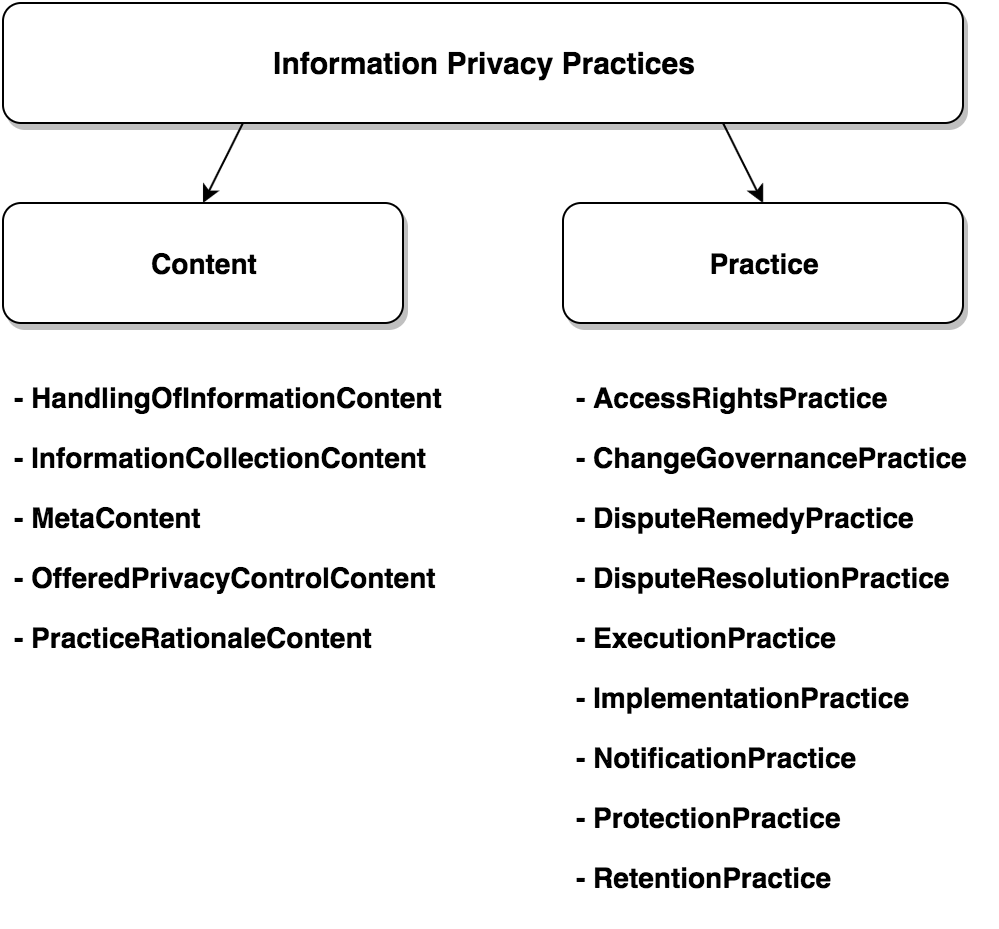
\includegraphics[keepaspectratio=true,width=350pt]{figures/IPP.png}
	\caption{Diagram of the hierarchy of information privacy practices, proposed by \cite{Dehling2016}.}
	\label{fig:informationPrivacyPractices}
\end{figure}

The top levels of the hierarchy, as seen in figure \ref{fig:informationPrivacyPractices}, are \textit{Content} and \textit{Practice}.
The \textit{Content} hierarchy level contains sub-hierarchy branches that express \ipp concerning the handling of information content, the information collection content, and meta content about information collection, information on offered privacy controls, and information on what purpose the \ipp were collected for.

We argue, if an information privacy practice is a circumstance that the user should be informed about, an information privacy practice expresses an information privacy risk to the app user.
But since not all of the enlisted \ipp express or imply an information privacy risk to app users, we review and extract the \ipp that are relevant in terms of posing and expressing a potential information privacy risk.
The classification of \ipp that bear or express an information privacy risk will be conducted by two researchers separately.
The results of the two researchers will be discussed to find common consensus about the classification.
We will further limit the \ipp by excluding \ipp that are known to be technically infeasible to detect via static code analysis of the app source code.
An example for such an exclusion is the information privacy practice \textit{InformationRetentionContent}, which captures, if an app provider carries out a certain information retention policy or not.\footnote{See \cite{Dehling2016}, p. 8.}
This is a feature that is undetectable by \sca and beyond the scope of app source code analysis.
An analysis of the app providers backend system would be necessary to ensure that the collection information is retained according to the app providers policy promise.

We include a full list of all \ipp in Appendix A including detailed comments on the technical limitations, if any, towards the \sca detection of each \ipp and wether they express a risk or not.

The following \ipp were identified as relevant to the \sca and further inspection within this thesis:

The complete hierarchy \textit{CH2} 'InformationSecurityContent' can be analysed via \sca including the \ipp 'SecurityDuringProcessingContent', 'SecurityDuringStorageContent' and 'SecurityDuringTransferContent'.
Partially supported will be the hierarchy \textit{CH3} 'InformationSharingContent'. Analysis will be applied to the containing \ipp \textit{CH33} 'SharingWithAdvertiserContent', \textit{CH34} 'SharingWithAggregatorContent', \textit{CH35} 'SharingWithAnalystContent', \textit{CH36} 'SharingWithDeliveryContent', \textit{CH37} 'SharingWithGovernmentContent', \textit{CH38} 'SharingWithOtherUsersContent', \textit{CH310}, \textit{CH311} 'SharingWithUnrelatedContent' 'SharingWithPublicContent' and \textit{CH312} 'SharingWithUserAuthorizedContent'.
The hierarchy \textit{CH4} 'InformationStorageContent' is relevant and can be analysed via static code analysis, as well as the hierarchies \textit{CI21} 'EnvironmentSensorContent', \textit{CI22} 'LocationSensorContent', \textit{CI23} 'UserSensorContent' and all their coherent sub-hierarchies.
For the hierarchy \textit{CI24} 'SoftwareUseSensorContent' only partial support for the sub-hierarchies \textit{CI242} 'CookiesContent' and \textit{CI243} 'SurveysContent' are feasible to be analyzed by static code analysis.
With the exception of one \ipp in the hierarchy level \textit{CI31} 'InformationFormContent' all other \ipp are relevant for this thesis: \textit{CI311} 'AudioInformationContent', \textit{CI312} 'ImageInformationContent', \textit{CI314} 'TextInformationContent' and \textit{CI315} 'VideoInformationContent'.
The next hierarchy level \textit{CI32} 'IdentifierContent' is fully relevant and all coherent sub-hierarchies will be analyzed.
More difficult to analyze via \sca will be the hierarchy level \textit{CI33} 'OperationalContent', because only two \ipp were identified as relevant to static code analysis: \textit{CI333} 'LocationContent', \textit{CI335} 'OnlineContactsContent' and \textit{CI336} 'PurchasesContent'.
Finally the hierarchy \textit{CI34} 'UserDetailsContent' is partially relevant, namely the \ipp \textit{I341} 'DemographicsContent', \textit{CI343} 'HealthContent', \textit{CI344} 'IdeologicalContent', \textit{CI345} 'PreferencesContent' and \textit{CI346} 'UserDeviceContent'.

All relevant \ipp and their \sca identification strategies will be explained further in chapter \ref{sssec:SCAP} of this thesis.

\section{Implementation and Evaluation of an Automated Information Privacy Risk Assessment Tool}

% Implementation of an Automated Information Privacy Risk Assessment Tool
\subsection{Implementing an Automated Information Privacy Risk Assessment Tool}

Our implementation of an \aiprat is structured in three phases.
In the first phase, Android APK files need to be downloaded to acquire the foundation of a static code analysis: the source code.
While APK files are binary representations of source code, it is necessary, in a second phase, to decompile to binary code back into actual source files.
The third phase is the analysis phase, where the information privacy risk assessment takes place.

\begin{figure}[h]
	\label{fig:implementationPhases}
	\centering
	\includegraphics[keepaspectratio=true,width=400pt]{figures/ImplementationFlow.png}
	\caption{Diagram of implementation phases of the \aiprat over time.}
\end{figure}

Figure 3-1 shows the implementation phases over time including the tools used within each phase. 
The tools will be described in greater detail within the following chapters.

% Download Phase
\subsubsection{Download Phase}

The download phase is the first of the three implementation phases and comprises the acquisition of Android APK files. 
The APK files hold the necessary Java source code that we will perform the \sca on.
Since this thesis emphases on Android mHealth apps, we used the repository database of \cite{Xu2015} as our main app data source.\footnote{This paragraph follows \cite{Xu2015}.}
\cite{Xu2015} list mHealth apps from the Apple AppStore\footnote{\url{https://itunes.apple.com}, visited 07/13/16} and Android PlayStore\footnote{\url{https://play.google.com}, visited 07/13/16} and update their repository quarterly by scraping the app stores.
The list contains information for example on the app's identifier, category in the app stores, description, email address of the developer, price and the user rating of the app.

We used the repository database to loop over the available mHealth app listings and included only the apps that were available for free, indicated by a price of \$0.00.
As soon as the package name of an app is gathered, the download of the \acs{APK} file can begin. 
While there is no official source to download \acs{APK} files for Android apps, a multitude of websites exist that host copies of \acs{APK} files to download for free.
Unfortunately, all of these websites implement mechanisms that make it impossible to browse and download the APK files programatically within a download script.
Instead, we used a open source Python implementation of an undocumented Google PlayStore \acs{API}.\footnote{\raggedright\url{https://web.archive.org/web/20140920061441/https://github.com/egirault/googleplay-api}, visited 05/12/16.} 
The undocumented part of the Google API allows users to download APK files.
Even though the project has not been maintained for four years, the software is still in working order.
The Python script authenticates to the Google API via the hardware ID of an Android smartphone or tablet and pretends to request data from this smartphone or tablet, even though the requests are sent from a desktop computer.
We used a real Android tablet to detect its hardware ID and authenticate the Google API requests with this hardware ID.
The main issue that has to be taken care of during the download phase is not to run into Google API limitations. 
Google allows an API user to only request a certain amount requests per time unit. 
After this limit is exceeded, the requests will just return a HTTP error code and no APK file will be downloaded.
In order to work around this circumstance, we ran our download script multiple times, always until the Google API returns error codes. 
We then waited a couple of hours and tried the download script again, which would pick up the download process where it had stopped on the last run.

% Decompilation Phase
\subsubsection{Decompilation Phase}

In order to decompile the amount of APK files available, it is necessary to automate the process. 
The automation script\footnote{\raggedright \url{https://github.com/thomasbrueggemann/AIPRAT/blob/master/decompile/decompile.sh}, visited 05/17/16.} uses a chain of tools to gather access to the source code files from an APK file.
The tools used to decompile the APK files follow closely the tools described and used by \cite{Enck2011}.\footnote{See \cite{Enck2011}, p. 5.}

In a first step, we use the tool \textit{dex2jar} to extract the \acs{JAR} file from the APK file.
The JAR file contains the java bytecode representations of the app which is just one part of the contents of an \acs{APK} file.
The next step is to extract resource files, such as the \textit{Android Manifest} file from the APK file.
The \textit{Android Manifest} contains meta information about the app in a structured XML format.\footnote{See for this and the next sentence \cite{xu2013}, p. 7 and \cite{Shabtai2010}, p. 331.}
The meta information include the package name of the app, the permissions the app requests, for example camera usage, internet access or geolocation usage.
The \textit{Android Manifest} file is therefore an important indicator at a high level view on activities within a given app.
In order to extract the \textit{Android Manifest} file from the APK file along with other resources such as images, icons, xml files or other files used within the app, we use the \textit{apktool}\footnote{\url{https://web.archive.org/web/20160617041519/http://ibotpeaches.github.io/Apktool/}, visited 06/17/16.}.
\textit{apktool} is a frequently updated Android reverse engineering tool that is used to extract resources from APK files.
Another important part of the extraction of resource files is retrieving the layout and localization files.
These files include information on the user interface components used within the app as well as text content for labels and text fields.
The text content will be used to train machine learning algorithms to classify features of the app, further described in the analysis phase section below.

At the core of the decompilation process is the usage of \textit{fernflower}\footnote{\url{https://web.archive.org/web/20150808204302/https://github.com/fesh0r/fernflower}, visited 05/24/16.}.
\textit{fernflower} is the recommended java decompiler by \cite{Enck2011}. 
They used the tool to decompile a test sample of apps and gained a significantly higher code recovery rate than by using other decompiling tools.\footnote{See \cite{Enck2011}, p. 6.}
An obstacle in decompiling java source code is obfuscation. 
Java developers can make use of a security feature called obfuscation that aims at hiding away the logic of java classes by renaming classes, variables and method names and disassembling the code into pieces that are difficult to read for an human interpreter.
The idea is to make it more difficult to retrieve and make sense of the original source code by decompiling the byte code.
\textit{fernflower} uses a renaming approach by assigning every obfuscated class with a new naming pattern. 
Member variables and methods will be automatically renamed and therefore provide an easier and more unique way of reading the source code.
Optionally the decompilation process can use an automatic code formatting tool called \textit{astyle}\footnote{\url{https://web.archive.org/web/20160422015538/http://astyle.sourceforge.net/}, visited 05/25/16.} to format the source code.
This helps humans to read the source code files more easily, since the formatting and indentation of all source code files is identical and therefore very structured.
Formatting the source code will help in the evaluation phase of this thesis to support the manual inspection the source code for \ipr by human researchers.

The expected result of the decompilation phase is a directory named after the package name of a given app that contains the resource files, including the \textit{Android Manifest} and the decompiled source code of the app.
The decompilation will be performed in order of file size.
The smaller the APK file the earlier it will decompiled.
This is due the fact that only APK files to a certain size can be analysed by the dataflow analysis tool, described in section \ref{sssec:SCAP}.

% Static Code Analysis Phase
\subsubsection{Static Code Analysis Phase} \label{sssec:SCAP}

The \sca phase is the main analysis phase of the thesis and uses the output of the previous decompilation phase to perform the static code analysis.
The \sca tool is implemented as a Java software project, since the used analysis libraries are implemented in Java and Android source code is written in Java too.
The output of the \sca Java project is an executable Java archive file called \textit{AIPRAT.jar} that can be executed in the command line terminal.
In order for \textit{AIPRAT.jar} to perform the \sca on APK files, two preparation steps are required.

The first preparation step is to run an Android data flow analysis tool over the APK files that extract potential data flows.
The data flow analysis is achieved with an open source tool called \textit{FlowDroid}, introduced by \cite{Arzt2014}.\footnote{See \cite{Arzt2014}, p. 259-269.}
\textit{FlowDroid} extends the Java optimization framework \textit{Soot}, which was already used by \cite{Enck2011} for post-decompilation optimization tasks.\footnote{See \cite{Enck2011}, p. 5.}
The data flow is analysed by scanning an intermediate byte code format provided by \textit{Soot} for so called 'sources' and 'sinks'.\footnote{See \cite{Arzt2014}, p. 264.}
A source is the origin of a data flow, for instance the user input of data via a textfield and a sink is the destination that data flows.
An example for a sink is a HTTP internet connection or a local log file.
\textit{FlowDroid} is also able to emulate Android lifecycle entry points.
While a regular Java program has a single entry point to start the application from, the \textit{main()} function, Android apps provide multiple entry points.
The entry points of an Android app are determined by the states an app can be in. 
It can for instance return from being in the background, do a fresh start and return from being offline.
All these entry points are being emulated by \textit{FlowDroid} into a single \textit{main()} function call.
The output of the data flow analysis is one XML file per analysed APK file that contains a list of sinks and the coherent sources of data flows to that sink.
The XML file will be parsed by the main \sca tool later on and the sink and source methods will be interpreted in the context of information privacy risks.

The machine learning text classifiers will be trained within the second preparation step.
During the \sca phase of this study, we will be making great use of the naive Bayes classifier.
A machine learning text-classifier classifies text segments into distinct categories. 
The categories are predefined in the training phase of the classifier, since every trained text segment is assigned with a training category.
These training categories are the categories the classifier can assign to new, previously unseen, text segments.
The incisive feature of a Bayes classifier is the fact, that it chooses to classify a category to a new segment of text by picking the most probable category.\footnote{For this and the following two sentences see \cite{Rish2001}, p. 41.}
A \nbc furthermore assumes that all categories are distinct and independent of each other. 
Even though this might not always be the case in a real life usage scenario, the \nbc still performs well enough for a wide range of use cases.

In the case of the \sca in this study, we will be using the \nbc to classify URLs into categories.
The categories that URLs can belong to, in the context of this study, are: advertisement, delivery services, government, instant-messaging, (data-) aggregation services, search engines and social networks.
While the set of categories might not complete in terms of all possible and available categories, it is sufficient for the classification of URLs within this \sca to classify into the mentioned category-set.
In oder for the \nbc to classify text into categories we trained a \nbc implementation with meta-information about URLs from the previously mentioned categories.
First, it was necessary to collect URLs for the categories to train the \nbc and we used a collection of \acs{URL}s from \textit{URLBlacklist.com}\footnote{\url{https://web.archive.org/web/20160617050003/http://urlblacklist.com/?sec=download}, visited 06/17/16.}.
\textit{URLBlacklist.com} provides URL lists for the categories advertisement, government, instant-messaging, search engines and social networks.
\textit{programmableweb.com} catalogues API descriptions including the service providers' URL.
We developed a program to automatically download and store the API directory for the two remaining categories, from \textit{programmableweb.com}.

Next, to acquire meta-information for all the URLs, we implement a downloader for the HTML source-code of all URLs and store the 'description' HTML-meta tag content in a file.\footnote{For this and the next sentence see \url{https://web.archive.org/web/20160404111603/http://www.w3.org/wiki/HTML/Elements/meta}, visited 07/13/16.}
The 'description' meta-tag contains a small amount of text, provided by the website owner, that describes the content or function of the website topic.
We use this 'description' meta-information to train the classifier with the associated categories.\newline

As soon as the preparation steps are finished, the main \sca tool is ready to perform the \ipr analysis.
We call the main \sca tool '\textit{AIPRAT}', short for \aiprat from here on.
The fundamental concept of \AIPRAT is to iterate over all available apps and apply a set of analysis operations, called 'strategies', to the source code of these apps.
A strategy tries to identify \iprfs by applying algorithms, for instance feature extraction or text search, to parts of the app source code.
There are two types of strategies in the AIPRAT: generic and specific strategies.

% Generic strategies
Generic strategies are strategies that contain algorithms that are configurable and usable by specific strategies.
Generic strategies are the core of the \aiprat and every non-generic strategy inherits or uses a generic strategy to accomplish its \ipr detection task.
The generic strategies of the \aiprat will therefore be explained in more detail.
In total the \aiprat contains eight generic strategies in the Java-package \textit{analyze.src.strategies}: DataFlowStrategy, ExistenceStrategy, InputStrategy, TraceBackStrategy, InformationCollectionStrategy, PermissionStrategy, ProviderUrlStrategy, and UrlCategoryStrategy.
\lstinputlisting[float=h, language=Java, label=listing:DataFlowStrategy, caption=Generic strategy DataFlowStrategy.java parses pre-extracted dataflow XML files]{DataFlowStrategy.java}
% DataFlowStrategy
The DataFlowStrategy parses the pre-extracted dataflow \acs{XML} from the \textit{FlowDroid} preparation phase and allows iterating over all identified dataflow sources and sinks.
Thereby, the DataFlowStrategy allows to pass parameters along that filter the sources and sinks for certain search words and provide feedback if the search words were found within sources and sinks.
The filtering if the searched sources of sinks are included can be seen in lines 5 and 13 of listing \ref{listing:DataFlowStrategy}.
% ExistenceStrategy
To find strings within the source code of an app, one can make use of the ExistenceStrategy.
The ExistenceStrategy is shown in listing \ref{listing:ExistanceStrategy}.
This generic strategy scans the full source code of an app and collects source code lines that match a given search pattern (See lines 5-6 of listing \ref{listing:ExistanceStrategy}).
\lstinputlisting[float=h, language=Java, label=listing:ExistanceStrategy, caption=Generic strategy ExistanceStrategy.java to find the existance of search words within source code]{ExistanceStrategy.java} 
% InputStrategy
The InputStrategy iterates over all \acs{XML} layout configuration files of an app. 
User interface controls that are displayed within an app are declared in these \acs{XML} layout configuration files.
The InputStrategy tries to identify all user input fields and therefore scans the layout files for the search terms 'EditText', 'AutoCompleteTextView', 'CheckBox', 'RadioButton' and 'RadioGroup' (see lines 4-5 of listing \ref{listing:InputStrategy}).
As soon as a user input field has been found, the InputStrategy extracts all meta information about this input field possible (see line 6 of listing \ref{listing:InputStrategy}).
The input fields meta information generally contain the user interface control 'id', a 'hint' field and a 'text' field. 
The meta information are collected and stored together with the input field information.
\lstinputlisting[float=h, language=Java, label=listing:InputStrategy, caption=The InputStrategy.java identifies user input fields and extracts their meta information]{InputStrategy.java}
% TraceBackStrategy
An important feature in static code analysis, especially for assessing information privacy risks, is the ability to trace data flows from a source to a sink.
With the help of the call graph construction feature of \textit{FlowDroid}, the TraceBackStrategy starts at a given set of start-sinks and traverses the call graph back until either a source is found or a given search pattern is matched, as seen in line 22 of listing \ref{listing:TraceBackStrategy}.
This allows consequent strategies to define a search pattern for data flows to specific sinks.
In the case of this thesis, we will mainly use the TraceBackStrategy to find data flows that end in a information collection scenario. 
We define information collection as a data flow that results in storing the information either locally on the device the app is run, or that results in sending the information to a remote server.
\lstinputlisting[float=h, language=Java, label=listing:TraceBackStrategy, caption=Excerpt of the generic strategy TraceBackStrategy.java to trace defined information sources to information sinks via dataflow analysis]{TraceBackStrategy.java}
% InputInformationCollectionStrategy
With making use of the InputStrategy and the TracebackStrategy, the InputInformationCollectionStrategy takes the user input fields analysis one step further and allows for information collection analysis.
\lstinputlisting[float=h, language=Java, label=listing:InputInformationCollectionStrategy, caption=The InputInformationCollectionStrategy takes the user input fields analysis and tries to identify information collection data flows]{InputInformationCollectionStrategy.java}
First, all user input fields are detected and stored, as seen in line 3 of listing \ref{listing:InputInformationCollectionStrategy}. 
In a second step, the InputInformationCollectionStrategy executes a TraceBackStrategy that starts at all available information collection sinks (local file storage and remote server connections) and traces back the call graph in an attempt to identify the user input field 'ids' within the call graph path (see lines 10-12 of listing \ref{listing:InputInformationCollectionStrategy}).
If a user input field is found, a data flow towards an information collection sink is identified and a potential \ipr is detected.
% PermissionStrategy
A less sophisticated approach is being used by the PermissionStrategy, shown in listing \ref{listing:PermissionStrategy}.
It is required for Android apps to declare permissions to use certain features, such as the \acs{GPS} location or internet access, within the 'manifest' file.\footnote{See \url{https://web.archive.org/web/20160425141027/https://developer.android.com/training/permissions/declaring.html}, visited 08/16/16}
The PermissionStrategy enables a search through these permissions by a given search pattern (see line 6 of listing \ref{listing:PermissionStrategy}).
\lstinputlisting[float=h, language=Java, label=listing:PermissionStrategy, caption=Generic strategy PermissionStrategy.java to find the existance of Android permissions declarations]{PermissionsStrategy.java}

The last two generic strategies concern the \acs{URL}s that are listed within the app source code and that are potentially target to information collection.
The ProviderUrlStrategy iterates over all extracted URLs found within the source code and checks how similar the URL host is in comparison to the app package name (see line 8 of listing \ref{listing:ProviderUrlStrategy}).
We observed that the package name often is similar to the hostname of the app provider or contains similar name parts. 
The ProviderUrlStrategy takes these potential sub-parts of the package name into account and returns a probability that a URL connection to the app provider is established (see line 12 of listing \ref{listing:ProviderUrlStrategy}.
\lstinputlisting[float=h, language=Java, label=listing:ProviderUrlStrategy, caption=Generic strategy ProviderUrlStrategy.java tries to identify URL connections to the app provider domain]{ProviderUrlStrategy.java}

Finally, the URLCategoryStrategy enables a search for a given category of URLs within the app source code.
All URLs are classified into distinct categories upon loading the app into the \sca tool via a machine learning text classification technique.
The classified categories are: 'ads', 'aggregation', 'delivery', 'government', 'instantmessaging', 'searchengines', 'socialnetworks' and 'storage'.
In order to check if a URL of a certain category exists, the URLCategoryStrategy iterates over all classified URLs and matches their categories to the search category, as seen in lines 7-8 of listing \ref{listing:URLCategoryStrategy}).
\lstinputlisting[float=h, language=Java, label=listing:URLCategoryStrategy, caption=The URLCategoryStrategy.java queries for the existance of URLs of a specific category within the app source code]{URLCategoryStrategy.java}

% Specific strategy
A specific strategy, on the other hand, targets the exploration of an \ipp directly and contains the \ipp hierarchy identifier, introduced by \textcite{Dehling2016}, in its Java-classname.\footnote{See \cite{Dehling2016}, p. 6.}
The Java-class \textit{analyze.src.strategies.CI213\textunderscore Strategy} contains a search pattern for the \ipp with the hierarchy identifier CI213, which refers to the \ipp Content (C) $\rightarrow$ InformationCollectionContent (I) $\rightarrow$ InformationCollectionSensorContent (2) $\rightarrow$ EnvironmentSensorContent (1) $\rightarrow$ MicrophoneContent (3).
Therefore a specific strategy may contain a combination of one or many generic strategies to try to identify the risk of the associated \ipp is posing through static code analysis.
In the example of the specific strategy \textit{analyze.src.strategies.CI213\textunderscore Strategy}, the class extends the generic strategy class \textit{analyze.src.strategies.ExistenceStrategy} and sets the search parameters of the \textit{ExistenceStrategy} to 'MediaRecorder.setAudioSource(' and 'MediaRecorder.AudioSource.MIC'.
The \textit{CI213\textunderscore Strategy} class scans via the parent-class \textit{ExistenceStrategy} all of the source code files off the app for source code that uses the Android microphone \acs{API}.

\begin{table}
	\begin{center}

	\begin{tabular}{ | p{4.8cm} | p{9cm} | }
	\hline
		ExistenceStrategy & CH21, CH23, CH310, CH311, CH312, CH33, CH35, CH38, CH43, CH44, CI212, CI213, CI214, CI221, CI222, CI223, CI231, CI242, CI243 \\ \hline
		InputInformationCollection-Strategy & CI321, CI322, CI323, CI324, CI325, CI326, CI341, CI343, CI344, CI345, CI346 \\ \hline
		InputStrategy & CI314 \\ \hline
		PermissionsStrategy & CH43, CH44, CI211, CI212, CI214, CI231 \\ \hline
		ProviderUrlStrategy & CH45 \\ \hline
		TraceBackStrategy & CH22, CH42, CH45, CI221, CI311, CI312, CI315, CI333, CI335, CI336 \\ \hline
		UrlCategoryStrategy & CH34, CH36, CH37, CH46 \\ \hline
	\end{tabular}
	\end{center}
	
	\caption{Specific strategies in relation to the generic strategies that they use} 
	\label{table:specStrategies}
\end{table}

% Explain specific strategies in more detail
In the following section we will introduce the specific strategies implemented in the \aiprat in greater detail.
Table \ref{table:specStrategies} displays and overview of the generic strategies in the first column and the specific strategies that make use of the coherent generic strategies in the second column.
The specific strategy classes in this chapter and in table \ref{table:specStrategies} are abbreviated with the \ipp hierarchy identifier of the matching strategy. 
\textit{CH21} for example stands for \textit{CH21\textunderscore Strategy.java} in this chapter.

% ExistenceStrategy
\textit{ExistenceStrategy}.
The generic ExistenceStrategy ist the most widely used strategy within the analysis tool.
% CH21
The strategy \textit{CH21} uses the ExistanceStrategy to check for the existance of the search words 'cipher' and 'crypt' that would indicate encryption during processing of data.
% CH23
Strategy \textit{CH23} uses the ExistenceStrategy twice to check if data transfers are secure. 
First strategy \textit{CH23} checks for the existence count of HTTP connections and second, it check for the existence count of HTTPS connections.
The result of \textit{CH23} is the ratio of \acs{HTTP} to \acs{HTTPS} connections.
% CH310 & CH312 & CH38
The strategies \textit{CH310}, \textit{CH311}, \textit{CH312} and \textit{CH38} try to identify a user initiated sharing of content with other users or the general public.
The strategies accomplish this by searching the source code of an app for triggering the Android sharing dialog window.
Additionally we search for methods that open sharing dialogs to three large social media networks, \textit{facebook}, \textit{twitter}, and \textit{Google+}.
% CH33
Strategy \textit{CH33} uses the generic ExistenceStrategy extensively to identify the usage of advertisement libraries within the app.
All search words are names of Android advertisement library identifiers and are derived from the analysis of Android ad libraries by \cite{Book2013}.\footnote{See \cite{Book2013}, p. 9.}
% CH35
In order to scan the source code of an app for the usage of analytics services, as stated in the hierarchy item \textit{CH35}, the strategy implementation for \textit{CH35} uses the ExistenceStrategy to check for analytics services and libraries search words.
The search words are derived from the open-source listing of Android libraries on https://android-arsenal.com in the category 'Analytics'.\footnote{\url{http://web.archive.org/web/20160514040053/http://android-arsenal.com/tag/5}, visited 07/03/16.}
% CH43 & CH44
\textit{CH43} and \textit{CH44} search for function names that indicate a writing of data to the internal or external storage of an Android device.
Internal and external storage can be a local database that every Android app instance can write to, the filesystem or a 'shared preferences' key value store, provided by the Android runtime.
Internal storage refers to storage of data on the devices' flash memory itself and external storage refers to storage of data on inserted storage mediums, such as storage card.
% CI212
Usage of the Android devices' internal camera is accomplished via a standardised \acs{API}.
In order to detect the usage of the internal camera, the \textit{CI212} strategy searches for the code snippets that are designated to launch the camera view inside of an Android app.
% CI213
A similar approach is used by the \textit{CI213} strategy, that aims at identifying the usage of the microphone recording by utilizing the ExistenceStrategy to find microphone calling function names.
% CI214
\textit{CI214} searches the source code for the usage of the Android near-field communication (\acs{NFC}) API, via the ExistenceStrategy.
The Android API has one particular method call to initiate a NFC connection, so detecting this feature via the ExistenceStrategy is effortless.
% CI221, CI222 & CI223
The strategies for \textit{CI221}, \textit{CI222} and \textit{CI223} utilize the ExistenceStrategy to detect wether the user's location is queried.
This can either happen by calling the Global Positioning System (\acs{GPS}) location, or by using the approximate location via the internet network connections of the device.
% CI231
A fairly new technique to smart-devices is the usage of a fingerprint sensor. 
This functionality is exposed via a single API entry-point in Android and can be detected by the \textit{CI231} strategy using the ExistenceStrategy.
% CI242
Also exposed via a single API entry-point is the ability to store and retrieve cookies\footnote{Cookies are pieces of information stored on the client device, accessible only by the provider that stored the cookie information until they expire. See \cite{Laudon2010}, p. 168.}.
Therefore the \textit{CI242} strategy can effortlessly detect the usage of such cookies within an app.
% CI243
More difficult is the detection of potential user surveys within an app.
\textit{CI243} uses the ExistenceStrategy to search the app source code for search words such as 'survey', 'audit' and 'syllabus'.

% InputInformationCollectionStrategy
\textit{InputInformationCollectionStrategy}. The following strategies try to identify dataflows from text input fields to information collection sinks.
% CI321
\textit{CI321} tries to identify dataflows from financial identification input fields. 
Financial identifier text input fields will be identified by using the search words: 'creditcard', 'cvc', 'iban', 'bic', 'bankaccount', 'bank', 'mastercard', 'paypal' and 'visa'.
If none of the search words are found within the identifiers of text input fields the certainty property of the result object is set to \textit{MEDIUM}.
This is because the list of search words might not be complete or the text input field are named in a non expressive way.
For example the text input fields might be named 'id=123456' instead of something expressive such as 'id=txtIBAN'.
The just explained certainty property value '\textit{MEDIUM}' for non-found input information collection dataflows holds true for the rest of the following strategies that use the InputInformationCollectionStrategy.
% CI322
Strategy \textit{CI322} tries to recognize government identifier dataflows within the app and uses the search words 'socialsecurity', 'insurance', 'tax', 'SSN', 'national', 'government' and 'identification'.
% CI323
\textit{CI323} only needs to identify the information collection of the name of the users, it utilizes the InputInformationCollectionStrategy with the search word 'name'. 
This automatically includes a search for 'surname' and for example 'middlename', since the InputInformationCollectionStrategy always performs a substring search within the text input field identifiers.
% CI324
The search words to identify an online contact of users are more definite.
Online contact information refers to the different ways users can be contacted online, for example via 'email', 'skype', 'facebook', 'twitter', 'chat' and many more.
\textit{CI324} uses the previously mentioned search words to identify dataflows of online contact information to information collection sinks.
% CI325
In contrast to the online contact information, the strategy for \textit{CI325} tries to identify information collection of physical contact information.
This refers to the address of users or their phone number.
% CI326
To identify users within an app itself, app providers implement their own unique user identifiers into the apps.
A unique user identifier could be a username, email address, and assigned Universally Unique Identifier (\acs{UUID}) or a password.
These unique user identifier information collection dataflows are detected by strategy \textit{CI326}.
% CI341
Strategy \textit{CI341} detects information collection of demographic information.
The search words for demographic information are derived from the survey recommendations for demographic standards from the German 'Statistisches Bundesamt'.\footnote{\raggedright See \url{https://web.archive.org/web/20151115091328/https://www.destatis.de/DE/Methoden/DemografischeRegionaleStandards/Fragebogen_schriftlich.pdf?__blob=publicationFile}, visited 07/05/16.}
% CI343
The strategy \textit{CI343} tries to identify users health information collection dataflows.
Here, the search words are derived from the manual review of mHealth apps by \textcite{Bruggemann2016}. 
The extensive health content search words are 'dosage', 'pill', 'blood', 'heart', 'bloodpressure', 'bloodsugar', 'heartrate', 'disease', 'symptom', 'weight', 'height', 'body', 'bmi', 'temperature', 'medical', 'doctor', 'calories', 'diet', 'sleep', 'carbon', 'hydrate', 'intake', 'haemoglobin', 'anaesthetic', 'urine' and 'hospital'.
% CI344
Ideological content, such as believes or membership of religious or political groups, information collection is detected by the strategy \textit{CI344}.
Input fields asking for membership of political parties for example, could be designed as option choice buttons and are captured by the InputInformationCollectionStrategy as well.
% CI345
Preferences of the users are difficult to capture, since preference-capturing input fields usually are connected to some sort of context, that users are asked their preferences about.
For the sake of this thesis, we will scan the input fields for expressions of preference, for example: 'like', 'dislike', 'favourite', 'favorite', 'preference' and 'prefered'.
We acknowledge that in case we did not find any preference capturing input field information collection, the certainty for this is at a level \textit{'LOW'}.
It is much more likely that we were unable to identify the information collection in that case.
% CI346
The last strategy using the generic InputInformationCollectionStrategy is the strategy for \textit{CI346}. 
Strategy \textit{CI346} tries to identify information collection of user device information, such as the Internet Protocol (\acs{IP}) address or the operating system name.

% InputStrategy
\textit{InputStrategy}. The generic InputStrategy is only used by a single specific strategy.
The strategy for \textit{CI314} tries to detect and list all of the input fields a user can input information into, within the app.
This is done by executing the InputStrategy, explained earlier in this chapter.

% PermissionsStrategy
\textit{PermissionsStrategy}.
% CH43 & CH44
The strategies for \textit{CH43} and \textit{CH44} check, as an additional condition, if a permission to write on external and internal storage is requested.
Only if a permission is declared, an app is allowed to use the coherent functionality of the Android API.
This is granted by the Android runtime.
% CI211
The strategy for \textit{CI211} relies solely on the generic PermissionsStrategy to identify the usage of Bluetooth functionality within the app.
An Android app is not granted access to the Bluetooth interface, if it does not declare the appropriate permission.
\textit{CI211} uses the PermissionsStrategy only, because Bluetooth interface APIs are not standardized and not easy to detect individually.
To 
% CI212 & CI214 & CI231
The previously described strategy implementations for \textit{CI212}, \textit{CI214} and \textit{CI231} behave in the same way as \textit{CH43} and \textit{CH44}.
They use the PermissionsStrategy as an additional condition, to detect the usage of the camera, near field communication \acs{NFC} and the fingerprint sensor.

% ProviderUrlStrategy
\textit{ProviderUrlStrategy}.
% CH45
The only specific strategy using the generic ProviderUrlStrategy is the strategy for \textit{CH45}.
It uses a list of all potential URLs that belong to the app provider, to identify information collection that sends data to the app providers servers.

% TraceBackStrategy
\textit{TraceBackStrategy}.
% CH45
Strategy \textit{CH45} uses, additionally to the ProviderUrlStrategy, the generic TraceBackStrategy.
It traces information collection flows to the previously detected app provider URLs.
% CH22
Dataflows that result in file storage on the internal flash drive or an external storage card can also be identified with the generic TraceBackStrategy.
The strategy for \textit{CH22} walks up the callgraph of all local storage collection sinks and checks if a function name containing the search words 'cipher' and 'crypt' was found along the way.
This would indicate that data stored on the local storage is stored in an encrypted way.
% CH42
Strategy \textit{CH42} tries to identify information collection at cloud storage providers.
Since it is virtually impossible to know, list and check for every possible cloud storage provider, the strategy searches for the word 'cloud' within dataflows that result in an information collection sink.
We acknowledge the low probability of actually finding a cloud storage dataflow with this technique by setting the certainty level of the result to \textit{'LOW'} by default.
% CI221 & CI333
A much higher success rate is promised by the standardized Android API to query the users location.
Detecting dataflows from these location queries to information collection sinks is done by the \textit{CI221} and \textit{CI333} strategies, mainly by searching for the usage of the 'LocationManager' object in Java.
The 'LocationManager' is the single point of entry to query the users location.
% CI311
A similar unambiguity is present for the detection of audio information collection.
While the callgraph is being traversed, strategy \textit{CI311} tries to identify function calls that contains the following search words: 'microphone', 'audio', 'recorder', 'mediarecorder', 'music' and 'sound'.
% CI312
The strategy for \textit{CI312} tries to detect the information collection of image information and therefore uses the search words 'picture', 'ACTION\textunderscore IMAGE\textunderscore CAPTURE', 'MEDIA\textunderscore TYPE\textunderscore IMAGE', 'CAPTURE\textunderscore IMAGE', 'image', 'setImageDrawable' and 'Bitmap'.
Central to image processing in Android is the 'Bitmap' object, as it is the binary representation of an image.
Detecting the usage of the 'Bitmap' object in an information collection callgraph path therefore yields a potential image information collection.
% CI315
The same holds true for strategy \textit{CI315}. 
In comparison to \textit{CI312}, \textit{CI315} tries to detect the information collection of video information.
Video processing in Android works immaturely different, than photo processing.
Instead of manipulating a 'Bitmap' object, as for the photo processing, videos are stored by the Android API and accessible via an uniform resource identifier (\acs{URI}).\footnote{\raggedright See \url{http://web.archive.org/web/20160425094249/https://developer.android.com/training/camera/videobasics.html}, visited 07/09/16}
Therefore the \textit{CI315} strategy can only detect video capturing information collection.
% CI335 
Strategy \textit{CI335} identifies information collection of the users contacts stored in his address book.
Querying the contacts via the Android API is always done via the 'ContactsContract' object.
The \textit{CI335} strategy can therefore easily detect information collection dataflows of users contacts by using the TraceBackStrategy.
% CI336
The last specific strategy to use the generic TraceBackStrategy is \textit{CI336} that tries to find information collection data flows on purchase information.

% UrlCategoryStrategy
\textit{UrlCategoryStrategy}.
As explained earlier in this chapter, the generic UrlCategoryStrategy preloads its training data of \acs{URL} classification into main memory at program start-time.
From then on, the UrlCategoryStrategy can be queried if certain URL categories are present within the currently inspected app. 
% CH34
Strategy \textit{CH34} searches for URLs that belong to a data aggregation service that potentially aggregates the users data.
% CH36
The \textit{CH36} strategy searches for URL connections to delivery services.
Delivery services can be postal service, package shipping or other logistic services.
% CH37
URLs to government institutions are identified by the \textit{CH37} strategy using the generic UrlCategoryStrategy.
% CH46
Finally, the \textit{CH46} strategy tries to detect URL connections to storage providers.
Storage providers refers to cloud storage or bulk data storage services that allow external data storage.

% Evaluation of an Automated Information Privacy Risk Assessment Tool
\subsection{Evaluation of an Automated Information Privacy Risk Assessment Tool}\label{chapter:evaluationMethods}

In order to evaluate how well the \aiprat is performing in comparison to a human researcher, we analyze a sample of three apps by two human researchers
The apps that will be chosen to be reviewed by human researchers will be the three apps with the most \ipr found by the \aiprat beforehand.
Each researcher is presented with the source code of the selected apps and the list of relevant information privacy practices to identify.
The task for each researcher is to identify as many \ipp as possibly by analyzing, searching and reading through the source code files. 
This will result in an overview comparison on how well the \aiprat performs in comparison to a human.

We acknowledge that a human app reviewer can almost find any \ipp risk within the app source code given enough time.
In order to find an appropriate time range that the human review should spend analyzing a single app, we looked at common review times of app stores today.
The Google PlayStore does not manually review newly uploaded apps, while the Apple AppStore does apply manual review to each and every app update.
The average time it takes for an app to pass the Apple AppStore review, which also includes waiting in a queue to be reviewed, is currently two days.\footnote{See \url{http://web.archive.org/web/20160513013009/http://appreviewtimes.com/}, visited 05/13/16.}
In order to keep the review times at a realistic level, a human app reviewer of our test sample apps should therefore not spend more than two days on analyzing a single app.

The reviewers will document their results in a tabular form, for each app.
For each of the relevant \ipp the reviewers will mark if they were able to detect the \ipr the \ipp poses or not.
Additionally they will report the certainty with which they feel that they detected the information privacy practice.
The certainty levels are \textit{LOW}, \textit{MEDIUM}, \textit{HIGH}.

A \textit{HIGH} certainty expresses, that the reviewers are very confident that they found the \ipp in question.
A \textit{LOW} certainty indicates that the reviewers found a potential indicator for an \ipp but is rather uncertain if this is indication expresses the full \ipp or if there are not any other indicators for the \ipp that were not found yet or are unfindable.
To express a neither high nor low certainty about a \ipp found, the reviewers can use a \textit{MEDIUM} certainty level.

Afterwards we will compare the results with the \ipr found by the \aiprat and draw conclusions from the comparison.
\section{Feasibility of Automated Information Privacy Risk Assessment}

\subsection{The Automated Information Privacy Risk Assessment of Free Android mHealth Apps}

\subsubsection{Download Phase}

\subsubsection{Decompilation Phase}

\subsubsection{\Sca Phase}

\subsection{Evaluation of the Auto- mated Information Privacy Risk Assessment Tool}
\section{Discussion}

The following chapter will discuss the results and limitations of this work and provide a possible insight into future research applications.

\subsection{Principal Findings}

First of all we want to discuss and highlight the reasons why 14 strategies did not report a 'found' result on the \ipr they were inspecting during the \sca phase.
We will follow the first row of table \ref{table:strategyResults}.
The Strategies CH34, CH36, CH37, CH38, CH43, CH45, CI213, CI222, CI223, CI321, CI322, CI344, CI345 and CI346 did not find any occurrence of an \ipr within the source code of the test sample apps.

Strategy CH34 and CH36 did not find any \ipr since the apps probably did not share information with aggregator and delivery services, known to the \aiprat in the \ml phase.
We argue that \mH apps are not the target group of delivery and aggregation services and are therefore not so widely used.

Strategy CH38 is not found, because the inter-app information sharing dialogue is not triggered from within the apps source code. 
Sharing between users is not a commonly used feature and the implementation of sharing between app users can be done in many different ways.
It is hard to capture this information privacy risk via static code analysis.
A \dca would be more appropriate in this context, to list and monitor the out- and inbound HTTP connections for data transfers.
The same holds true for CH45.
No data connections to the app provider were detected. 
Our approach within the \aiprat was to construct the potential provider url beforehand and then executing the detection analysis.
Again, with using a \dca the app provider URL could probably be detected more reliable.
The \dca would list all URLs that the app connects to and similarities with the app provider name can be computed or even derived.
The reason we did not use a \dca within this thesis is the premise to be able to analyse \mH apps fast, independent from a runtime and at low costs.

Strategy CH43 tries to detect data storage on internal storage media by, among another factor, looking at the permissions the Android app declares to use.
Looking at the current Android documentation for the usage of permissions, the 'WRITE\_ INTERNAL\_ STORAGE' permission that strategy CH43 uses seems to be deprecated and no longer used.\footnote{\raggedright See \url{https://web.archive.org/web/20160713184910/https://developer.android.com/reference/android/Manifest.permission.html}, visited 08/17/16.}
This could be an indicator for the results of strategy CH43.

Strategy CI213 might not be detectable within \mH apps because recording audio via the built in microphone is not a typical use case of a \mH app.

Strategy CI213 tries to identify just that, the information collection of the Android microphone API usage.
For Strategy CI222 it is clearer why the \ipr is not detected within the apps source code.
It tries to detect the usage of the users location via the network connection by interpolating the user position between cellphone towers.\footnote{\raggedright See \url{https://web.archive.org/web/20160626232714/https://developer.android.com/reference/android/location/LocationManager.html}, visited 08/17/16.}
This mode of location data acquisition is not very accurate in comparison to using the Global Positioning System (GPS) position.
It is very likely that apps that are interested in the users location just use the GPS location. 
It might also be the case that \mH apps do not use the users location that often.
The same holds true for strategy CI223, since Android does not distinguish between the location acquisition via WiFi or the cellphone tower interpolation.
Android merges the two concepts under the 'NETWORK\_ PROVIDER' mode for location acquisition.

Since strategy CI321 aims at identifying the information collection of financial identifications of the app users, we conclude that \mH are not prone to collecting financial information of users.
Their main function might be to deliver added value to the health knowledge of the user and monetization is only a perceived secondary goal.
With the advent of in-app purchasing options, the need to ask users for their financial information has potentially changed a lot.
Apps can implement purchases within an app by using in-app purchase APIs of the operating system.\footnote{\raggedright For this and the following sentence, see \url{https://web.archive.org/web/20160812084756/https://developer.android.com/google/play/billing/billing_overview.html}, visited 08/17/16.}
These APIs encapsulate the purchase process and streamline the purchase action, since the financial identification is globally stored at the app store site.

We further argue that only few \mH apps collect ideological information on the users, such as religious views, political tendencies or believes. 
Therefore, strategy CI344 that tries to detect these ideological information collection is not found within our test sample of \mH apps.

The same argument can be used to explain the missing of \ipr within the sample apps of the strategies CI345 and CI346.
Hardware information on the users device and user preferences, such as likes or dislikes, are not the target information domain of \mH apps.

After discussing the reasons why 14 strategy implementations did not result in an \ipr found, we will take a look at the degree to which the assessment of information privacy risks for \mH apps can be automated via static code analysis.

In order the evaluate the degree to which the assessment of information privacy risks for \mH apps can be automated via static code analysis we compared the \ipr found results of the \aiprat with the results from the human researchers.

While it is clear that the computer is faster in processing files and scanning the file's content, the human has at least one advantage over the computer: understanding or estimating context of source code based on his experience.

We were unable to implement a \ml approach to identify all information privacy risks.
Especially difficult is, for instance, the identification of previously unknown analytics or advertisement libraries.
The \ml approach was unfeasible due to the missing context and meta information for the software to learn from.
Using just a line of code to teach the \ml implementation a pattern is not sufficient, since there is no further meta information that could be compared by the algorithm.
Looking at the \ml of \textcite{Shabtai2010}, the problems regarding the context in our approach become clearer.
\textcite{Shabtai2010} used the complete text body of all Java code files within each app to train the \ml classifier to distinguish between two app categories.\footnote{See \cite{Shabtai2010}, p. 330.}
An analytics or advertisement library can be named virtually anything, without any pattern.
Therefore, the computer needs a list of possible analytics and advertisement libraries in order to identify them in a static code analysis.
We used analytics and advertisement libraries as an example of two information privacy risks here, the \ml approach problems apply to other \ipr strategies as well.

The context interpretation skills of humans became even more obvious, during the manual review by the two researchers.
The computer, for instance, did not identify the \ipr 'InformationCollectionTypeContent' $\rightarrow$ 'HealthContent' implemented in strategy \textit{CI343} for the test app 'com.siyami.apps.patientregister' because the matching source code was obfuscated.\footnote{See coherent row for \textit{CI343} of app 'com.siyami.apps.patientregister'  in table of Appendix B.}
The human researchers on the other side were able to identify the 'HealthContent' \textit{CI343} \ipr because they were able to interpret the context in which the obfuscated code was used, by interpreting source code comments for instance or interpreting the screen context.

Another example where the human reviewer is superior to the computer in identifying \ipr with a \sca is the strategy \textit{CI326} 'OwnUniqueIdentifierContent'.
A unique identifier can be implemented in many shapes and it is therefore especially difficult to detect.
A human reviewer has the advantage to interpret variable names and the context that variables are used in to identify a unique user.
A unique user identification can be a randomly generated string, the email address of the user or any other unique feature that is unique to a single user.

Additionally, it is difficult for the computer software to generalise concepts.
The human reviewer can estimate how likely it is, that a higher hierarchy level \ipp bears an information privacy risk within the current app, by understanding the context.
In order for the computer to decide weather a high-level hierarchy is found, it has to check all the containing sub-hierarchy \ipp first.
The human reviewer has, yet again, the benefit of context interpretation to generalise risk factors.
\newline\newline
We have met the first sub-objective, declared in chapter \ref{chapter:Objectives}, by stepping through the \ipp provided by \textcite{Dehling2016} and extracted the \ipp that potentially bear an information privacy risk to \mH app users.
This progress was documented in chapter \ref{chapter:Relevant}.

We developed strategies for each of the relevant \ipp to be identified within the source code of \mH apps in chapter \ref{sssec:SCAP}, in order to achieve the second sub-objective.

The final and third sub-objective is to compare the results of the human source code review with the results of the \aiprat and highlight the differences in results between human and computer.
The discussion of these results took place in this chapter.

Finally, in order to find a reasonable way to express the degree to what the assessment of information privacy risks can be automated, we will apply the following process.
At first, we identified 55 of the \ipp to be relevant for posing an information privacy risk. 
45 of these \ipp were able to be implemented within the \aiprat and therefore the 'implementation rate' is:
\begin{equation}
	\frac{45}{55}=0.818
\end{equation}

In a second step we will use the results from table \ref{table:reviewerResultsCertainty} to generate an index number that expresses the performance of the computer in relation to the human in assessing information privacy risks.
We argue that the cumulative certainty levels (CCL) express the degree to which  the information privacy risk assessment of \mH apps more accurately than the simple sum of 'found' \ipp for each app.
For every row in table \ref{table:reviewerResultsCertainty}, we are taking the maximum number of the CCL as 100\% and calculate the fraction percentage that the computer found from the 100\%.
We will then take the average value of the just calculated fractions.
This would result in a 'detection rate' of:
\begin{equation}
	\frac{\frac{11.25}{12.75} + \frac{9.25}{9.25} + \frac{9.75}{9.75}}{3} = 0.96
\end{equation}

For the sake of the calculation of this degree value, we will not take the fact that we were only able to decompile and analyze a fraction of the downloaded apps, due to hardware limitations, into account.
We will not lower the degree based on the percentage of apps that was downloadable or able to be analyzed by \textit{FlowDroid}.
These limitations can possibly be eliminated in future research by applying more computation power and time to the analysis.
But, to combine the 'implementation rate' and the 'detection rate', we will take the average of the two values, which results in:

\begin{equation}
	\frac{0.818 + 0.96}{2} = 0.889
\end{equation}

We therefore conclude, that the degree to which an \aiprat is feasible or implementable is 88.9\%, compared to a manual \sca by a human researcher.
A completely automated information privacy risk assessment is "desirable but unrealistic today" \footnote{\cite{Knorr2015}, p. 7.}.

\subsection{Contributions}

As a contribution of the results of this thesis, we propose our implementation of an \aiprat that works in a three step process.
The tool downloads, decompiles and analyses an APK file of an app to perform the information privacy risk analysis.

In an attempt to evaluate the outcome of the \aiprat we compared the results of a \sca of two human researchers to the results of the computer.

The contribution of this thesis is the increase of knowledge, that an automated information privacy risk assessment is possible up to a degree of 88.9\%, compared to a manual \sca by a human researcher.

\subsection{Limitations}\label{chapter:Limitations}

The most effecting limitation during this study was the time constraint.
The time constraint applies to the time we were able to implement the \aiprat as well as the time we were able to run the tool afterwards.
It would be possible to run the analysis for longer and on more apps, with more time available and a budget for computation resources.

Developing such a holistic approach on the identification of the degree a \sca might be usable to identify \ipr within \mH apps automatically resulted in cutting the implementation of the \ipr detecting strategies short, in some cases.
While some \ipr are currently detected by using search words and scanning the source code, it would be ideal to create a tool that automatically learns search words form a training set and applies this knowledge to further app analysis.
In order to develop a machine learning approach on detecting features or patterns in source code files, it is always necessary to have meta information on the source code lines available.
We applied a machine learning approach to classify URLs that are called from within the app into categories. 
We were able to acquire meta information on the URLs (the description HTML text) that allowed the classification algorithm to learn the description text words for each URL and category.
For a Java code line there is no such thing as meta information or even the ability to break a code line into acceptable, 'learnable' features.
In order to identify, for instance, analytics libraries it is not enough to break the source code lines of the analytics library call up, 'learn' the source code line parts and apply the 'knowledge' to further lines.
Analytics libraries, for instance, can be called in many ways and their \acs{API}s are not uniform.
Therefore we were unable to implement more machine learning applications other than the URL classification.

Furthermore, the output of the \aiprat is a rather technical accumulation of the \sca strategy outputs.
The results have not been aggregated into a single information privacy index or a more user friendly communication or interpretation of the information privacy risks detected.

\subsection{Future Research}

Since this study targeted more than one field of interest, future research can target a manifold of improvements.

First of all, the provision of source code files could be improved. 
Currently no access to the binary source code files of other app store provider than the Google Play Store are possible.
Future researchers could organise partnerships with other app store providers to gain legal access to their app source code files.

Another major factor of improvement is the computation power and time that we were able to spend on the decompilation and analysis phase.
Future researchers could use dedicated computers to run the decompilation and analysis phases or even develop this software, or the memory-critical \textit{FlowDroid} toolset, further into a cluster application that runs on multiple machines.
This could allow future researchers, with less of a time-constraint, to run the analysis on more apps and potentially gain additional insights from the results.

We tried to use as many external and comprehensive resources for finding search words, if strategies called for such.
For example the strategy for the information privacy practice hierarchy \textit{CH35} 'SharingWithAnalystContent' uses search words derived from a collection of Android analytics apps.
These search words can be further extended, or, as mentioned in the previous chapter \ref{chapter:Limitations}, extended into a machine learning approach. 
Future research could enhance the current implementation in a way that it proposes and highlights risky parts of the source code to be reviewed by a human additionally.

The approach of this study can also be seen as a first step towards the larger goal of providing transparency to the \ipr of, especially mHealth, apps.
The outcome of the \aiprat could be incorporated into a user interface, similar to the user interface proposed by \textcite{Bruggemann2016}\footnote{See \cite{Bruggemann2016}, p. 1-10.}.
In this context, future research could inspect the implications and the impact such a detailed \ipr analysis has on the users of apps and app stores, in a user study.

We would also like to encourage future researchers to address the implications an integration of automated information privacy risk assessment may have on the app stores and the submitting of apps to the stores for developers.
Future research could analyse what the effects are if an app store, for instance the Google PlayStore, implements an automated \ipr analysis tool that performs a \sca right after a developer submitted an app and transparently communicates the information privacy risks found within the source code.

Regarding the \aiprat itself, future research can improve the tool as well as the search words used within the various specific strategies, explained in section 3.1.3.
Future researchers could develop test cases to automatically test the whole proposed workflow of the three phases, in section 3.1 as well as individual test cases for each of the implemented strategies.

\subsection{Conclusion}

This master thesis is a practice-oriented research-work that tries to answer the question to what degree an information privacy risk assessment of \mH apps can be automated by implementing such a tool and testing the feasibility.

In the emerging market of \mH apps, the focus on information privacy risks is growing.
Based on the large amount of apps in the app stores and the continuous growth, manual review is infeasible.
Yet, to the best of our knowledge, no study thus far linked a holistic information privacy risk assessment of \mH apps with automatic \sca approaches.
In this thesis, we introduced an \aiprat that is, with small human configuration, able to download, decompile and analyse Android \mH apps.

We find that the information privacy risk assessment of \mH apps can be automated to a degree of 88.9\%.
The computed degree includes the implementation rate, of how many \ipr can be identified by a \sca strategy, and the detection rate, with which certainty the \ipr were identified.

The results of this thesis, the \aiprat source code and the insights on the limitations and achievements of the \sca usage, can be seen as the foundation for future research to build on.
With dedicating more resources to the points mentioned in the limitation chapter \ref{chapter:Limitations} future researchers can enhance the \aiprat even further.
\newpage

% --------------------
% References
% --------------------
\newpage
\patchcmd{\bibsetup}{\interlinepenalty=5000}{\interlinepenalty=10000}{}{}
\printbibliography[title={References}]
\addcontentsline{toc}{section}{References}
\newpage

% ---------
% Appendix
% ---------
\section*{Declaration of Good Scientific Conduct}
\addcontentsline{toc}{section}{Declaration of Good Scientific Conduct}

Hiermit versichere ich an Eides Statt, dass ich die vorliegende Arbeit selbstständig und ohne die Benutzung anderer als der angegebenen Hilfsmittel angefertigt habe. 
Alle Stellen, die wörtlich oder sinngemäß aus veröffentlichten und nicht veröffentlichten Schriften entnommen wurden, sind als solche kenntlich gemacht. 
Die Arbeit ist in gleicher oder ähnlicher Form oder auszugsweise im Rahmen einer anderen Prüfung noch nicht vorgelegt worden.
\vspace{15mm}
\begin{flushleft}
    Viersen, den 01. September 2016
\end{flushleft}
\vspace{30mm}
I hereby attest that I completed this work on my own and that I did not employ any tools other than those specified. 
All texts literally or semantically copied from other works are attributed with proper citations. 
This work has not been submitted in identical or similar form for any other exam, assessment, or assignment.
\vspace{15mm}
\begin{flushleft}
    Viersen, September 1st, 2016
\end{flushleft}
	
\section*{Curriculum Vitae} 
\addcontentsline{toc}{section}{Curriculum Vitae}

\begin{flushleft}

% Persönliche Angaben
\begin{tabular}{p{11em} p{10em} p{10em}}
    \multirow{5}{*}{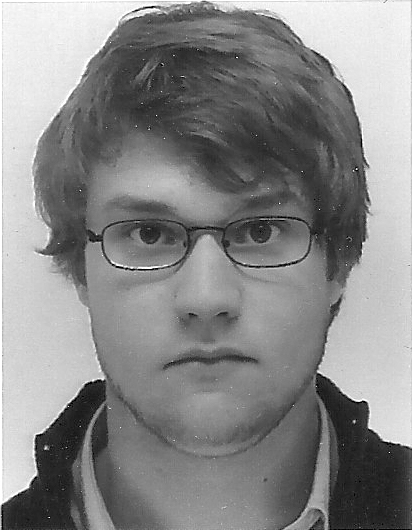
\includegraphics[width=40mm]{figures/passfoto.jpg}} & \textbf{Persönliche Angaben} & \addspace \\
    & Name: & Thomas Brüggemann \\
    & Anschrift: & Hoferkamp 9, 41751 Viersen \\
    & Geburtsdatum und -ort: & 31.08.1989 in  Viersen \\
    & Familienstand: & verheiratet \\
\end{tabular}

\vspace{2.7em}

% Ausbildung
\begin{tabular}{p{11em} p{22.5em}}
    \textbf{Schulische Ausbildung} & \addspace \\
    1997 - 2001 & Katholische Grundschule Boisheim \\
    2001 - 2009 & Bischöfliches Albertus-Magnus-Gymnasium in Viersen, Abschluss: Abitur \\
\end{tabular}

\vspace{0.5em}

% Grundwehrdienst
\begin{tabular}{p{11em} p{22.5em}}
    \textbf{Grundwehrdienst} & \addspace \\
    07/2009 - 04/2010 & \raggedright Wehrdienstleistender, Luftwaffe - JaboG 31 "Boelke", Kraftfahrer vom Dienst, Fliegerhorst Nörvenich \\
\end{tabular}

\vspace{-1.5em}

% Studium
\begin{tabular}{p{11em} p{22.5em}}
    \textbf{Studium} & \addspace \\
    10/2010 - 03/2014 & Universität zu Köln, Wirtschaftsinformatik, Bachelor of Science \\
    10/2014 - 09/2016 & Universität zu Köln, Information Systems, Master of Science
\end{tabular}

\vspace{0.5em}

% Beruflicher Werdegang
\begin{tabular}{p{11em} p{22.5em}}
    \textbf{Beruflicher Werdegang} & \addspace \\
    05/2010 - 09/2012 & Thomas Trefz Consulting, Köln, Softwareentwicklung im Bereich Microsoft .NET \\
    10/2012 - 10/2014 & Beister Software GmbH, Aschaffenburg, Softwareentwicklung im Bereich Microsoft .NET \\
    10/2014 - heute & Selbstständiger Softwareentwickler und IT-Berater
\end{tabular}

\end{flushleft}

\end{document}
